\documentclass[pdftex,12pt,a4paper]{article}
\pdfpagewidth 8.5in
\pdfpageheight 11.6in
\linespread{1.3}
\usepackage{anysize}
\marginsize{2.5cm}{2.5cm}{2.5cm}{2.5cm}

\usepackage[utf8]{inputenc}
\usepackage[T1]{fontenc}
%\usepackage[magyar]{babel}
\usepackage{indentfirst}
\usepackage{amsmath}
\usepackage{subcaption}
\usepackage{float}
\usepackage{graphicx}
\usepackage{braket}
\usepackage{tensor}
\usepackage{hyperref}

%\usepackage{listings}

\DeclareMathOperator{\Ai}{Ai}
\DeclareMathOperator{\Bi}{Bi}
\DeclareMathOperator{\Aip}{Ai^\prime}
\DeclareMathOperator{\Bip}{Bi^\prime}
\DeclareMathOperator{\Ti}{Ti}
\DeclareMathOperator{\ctg}{ctg}
\DeclareMathOperator{\sgn}{sgn}
%\DeclareMathOperator{\max}{max}
\let\Im\relax
\DeclareMathOperator{\Im}{Im}
\DeclareMathOperator{\Tr}{Tr}
\newcommand{\op}[1]{\hat{#1}}
\newcommand{\norm}[1]{\left\lVert #1 \right\rVert}
\newcommand*\Laplace{\mathop{}\!\mathbin\bigtriangleup}

\newcommand{\aeqref}[1]{\az{\eqref{#1}}}
\newcommand{\Aeqref}[1]{\Az{\eqref{#1}}}

%---------------------------------------------------------------------------------------------------------------------
\usepackage{fancyvrb,newverbs,xcolor}

\definecolor{cverbbg}{gray}{0.93}

\newenvironment{cverbatim}
 {\SaveVerbatim{cverb}}
 {\endSaveVerbatim
  \flushleft\fboxrule=0pt\fboxsep=.5em
  \colorbox{cverbbg}{\BUseVerbatim{cverb}}%
  \endflushleft
}
\newenvironment{lcverbatim}
 {\SaveVerbatim{cverb}}
 {\endSaveVerbatim
  \flushleft\fboxrule=0pt\fboxsep=.5em
  \colorbox{cverbbg}{%
    \makebox[\dimexpr\linewidth-2\fboxsep][l]{\BUseVerbatim{cverb}}%
  }
  \endflushleft
}

\newcommand{\ctexttt}[1]{\colorbox{cverbbg}{\texttt{#1}}}
\newverbcommand{\cverb}
  {\setbox\verbbox\hbox\bgroup}
  {\egroup\colorbox{cverbbg}{\box\verbbox}}
%---------------------------------------------------------------------------------------------------------------------
%\frenchspacing
\begin{document}

	\centerline{\bf\LARGE General relativistic ray tracing}\vskip0.4truein
	\centerline{\LARGE Computer simulations in physics}\vskip0.4truein
	\centerline{\Large\sc Kürti Zoltán}\vskip0.10truein
	%\centerline{\includegraphics[scale=0.5]{./elte_cimer_color.pdf}}
	\vskip0.4truein
	\centerline{\Large{\sc{2021.10.22.}}}
	\thispagestyle{empty}
	\newpage
	\tableofcontents
	\newpage
	\section{Introduction}
		Modeling light transport in the framework of general relativity is an important topic in physics. Modern observatories allow multiple different measurements that can be compared to predictions of general relativity about light transport. \cite{quasar, test1} These type of measurements are among the most important experimental confirmations of general relativity. Gravitational lensing can generally be divided into two categories, strong and weak gravitational lensing. In our work we focus on strong gravitational lensing using numerical methods. This category of lensing is important for understanding observations about distant massive compact objects like neutron stars and black holes. Resolution of light originating from the strongly lensing region of nearby supermassive black holes is now possible thanks to the Event Horizon Telescope collaboration. 
	\section{Theoretical background}
	\subsection{Light rays}
		We will use $(+,-,-,-)$ sign convention during this project. In the document Greek indices run from 0 to 3, latin indices in general run from 1 to 3 except when they index a vierbein vector in which case they run from 0 to 3, the 0th vector being timelike.
		
		We modeled light in the geometric optics approximation, meaning light is descried by light rays. These light rays in general relativity correspond to null geodesics.
		
		The equation to be solved is therefore
		\begin{equation}
			\frac{\mathrm{d}^2\tensor{x}{^\mu}}{\mathrm{d} t^2} + \tensor{\Gamma}{^\mu_\alpha_\beta}\frac{\mathrm{d}\tensor{x}{^\alpha}}{\mathrm{d}t}\frac{\mathrm{d}\tensor{x}{^\beta}}{\mathrm{d}t}= 0,
			\label{geodesic}
		\end{equation}
		with initial conditions $x^\mu(0) = x_0^\mu$ and $\frac{\mathrm{d}\tensor{x}{^\mu}}{\mathrm{d} t}(0) = \tensor{v}{^\mu}$ where $\tensor{v}{^\mu} \tensor{v}{_\mu} = 0$ in order for the geodesic to be null. In this case we want to integrate this equation backwards in time since the information we have is the direction and position of the ray when it hit the camera. From this information we have to determine the first intersection of the light ray of an object of interest that we want to visualize. This can be achieved with forward integration methods using $v_0^0 < 0$.
	\subsection{Observers in general relativity}
		Observers or cameras in this case can be described with a point $p_0$ in spacetime and a vierbein $\tensor{e}{_a^\mu}$ at that point $p_0$. $\tensor{e}{_0^\mu}$ is a future timelike vector, corresponding to the 4-velocity of the observer. The rest of the four vierbein vectors represent the $x$ $y$ and $z$ coordinates of the observer. For the camera $x$ is the forward direction, $y$ is the up direction and $z$ is the right direction. These four vectors have to be orthogonal to each other, this way they describe a local coordinate system that is like the usual $(t,x,y,z)$ coordinate system used in special relativity:
		\begin{equation}
			\tensor{e}{_a^\mu}\tensor{e}{_b_\mu} = \tensor{\eta}{_a_b}
			\label{viebein}
		\end{equation}
		where $\tensor{\eta}{_a_b} = \mathrm{diag}\left(1,-1,-1,-1\right)$ is the metric tensor from special relativity in $(t,x,y,z)$ coordinates.
		
		Int this local coordinate system the construction of a virtual screen is possible knowing the screen resolution and field of view. Choosing a pixel on this screen the corresponding light ray will have spatial velocity components equal to that of the pixel's, and a negative time component chosen such that the velocity vector is a past null vector. This velocity together with the position of the camera are the initial conditions of the geodesic equation. This formalism automatically includes all special relativistic effects on the directions of light rays, relativistic aberration is well illustrated by images generated based on this camera system.
	\subsection{The Schwarzschild black hole}
		Einstein's equations can be solved for the vacuum case assuming spherical and time translation symmetry. This solution is called the Schwarzschild solution. Many coordinate systems are used to describe this solution. In our choice the metric tensor is
		\begin{equation}
			ds^2=\left(1-\frac{2GM}{rc^2}\right)c^2dt^2 - \frac{1}{1-\frac{2GM}{rc^2}}dr^2 - r^2d\theta^2 - r^2\sin^2\left(\theta\right)d\phi^2.
		\end{equation}
		This choice has the advantage that the formulas are easy to compute, everything is expressed in elementary functions and that for large values of $r$ it is a good match for the usual spherical coordinates, which will be useful to approximate the intersection of light rays with the celestial sphere. The main disadvantage of theis coordinate system is that it is singular at the event horizon, meaning that numeric solutions can't cross it and the stepsize required to remain precise approach 0. This is not a problem if the camera stays outside the event horizon.
		
		The non-zero components of the Christoffel-symbols up to symmetry in the last two indices are
		\begin{equation}
			\begin{aligned}
				\tensor{\Gamma}{^t_r_t} &= -\tensor{\Gamma}{^r_r_r} = \frac{r_s}{2r\left(r-r_s\right)}\\
				\tensor{\Gamma}{^r_t_t} &= \frac{r_s\left(r-r_s\right)}{2r^3}\\
				\tensor{\Gamma}{^r_\phi_\phi} &= \left(r_s-r\right)\sin^2\left(\theta\right)\\
				\tensor{\Gamma}{^r_\theta_\theta} &= r_s - r\\
				\tensor{\Gamma}{^\theta_r_\theta} &= \tensor{\Gamma}{^\phi_r_\phi} = \frac{1}{r}\\
				\tensor{\Gamma}{^\theta_\phi_\phi} &= -\sin\left(\theta\right)\cos\left(\theta\right)\\
				\tensor{\Gamma}{^\phi_\theta_\phi} &= \cot\left(\theta\right).
			\end{aligned}
		\end{equation}
	\section{Program description and results}
		The program was written in C++, and uses only two external libraries, LibTIFF to write images to disc and OpenMP to parallelize for loops. The code can be downloaded from \url{https://github.com/KurtiZoltan/CompSim1}.
		
		The program was designed to be easily extendable, any spacetime geometry can be represented just by implementing a child class of the pure virtual Spacetime class. An arbitrary number of displayable objects can be used. Their geometry is defined by scalar valued functions of the spacetime coordinates, negative values indicating the inside of the objects and zero the surface. The pixel color of a hit is calculated by another function that is a function of the spacetime coordinates along with the velocity vector of the light ray at the time of the hit. These two functions are provided by the user and added to an object of class Objects containing data relevant to intersection calculations.
	\subsection{General structure}
		The user has to provide an implementation of the abstract class Spacetime, provide the intersection and color functions corresponding to each object, give some initial data about the reference frame and camera. After these steps the program is ready to render the image seen by the camera.
	\subsubsection{Vierbein calculation}
		First based on the initial data provided to the reference frame, the proper vierbein corresponding to the observer is calculated. This requires the metric tensor with which using orthogonal projections the \ctexttt{lookAt} vector is projected with the \ctexttt{time} vector to obtain the \ctexttt{forward} vector. The \ctexttt{up} vector is both projected with the \ctexttt{time} and \ctexttt{forward} vectors to obtain the true \ctexttt{up} vector. Finally the four basis vectors are all projected with all three previous vectors, \ctexttt{time}, \ctexttt{forward}, \ctexttt{up}. The biggest norm out of theses is choosen for maximal numeric accuracy. This vector is parallel to the \ctexttt{right} direction. The sign is determined by the determinant of the four vectors, this ensures that the vierbein is right handed. As a final step the vectors are normalized, this completes the calculation of the vierbein representing the observer.
	\subsubsection{Initial condition generation}
		The next step is the determination of the initial conditions corresponding to the pixels of the camera. The initial position is dimply the position of the camera, while the initial velocity is calculated according to the following formula:
		\begin{equation}
			\ctexttt{dir} = \frac{\ctexttt{forward} + u\ctexttt{up} + r\ctexttt{right}}{\sqrt{1 + u^2 + r^2}} - \ctexttt{time},
		\end{equation}
		where $u$ and $r$ represent the pixel coordinates calculated based on the field of view and the resolution of the image,
		\begin{equation}
		\begin{aligned}
			\ctexttt{r} &= \tan\left(\frac{\ctexttt{FOV}}{2}\right)\left(\frac{\ctexttt{2x}}{\ctexttt{width} - 1} - 1\right)\\
			\ctexttt{u} &= \tan\left(\frac{\ctexttt{FOV}}{2}\right)\left(\frac{\ctexttt{2y}}{\ctexttt{height} - 1} - 1\right)\frac{\ctexttt{height}}{\ctexttt{width}}\\.
		\end{aligned}
		\end{equation}
		This means that the time component of the light ray in the observer's reference frame is always $1$, wich will be useful when calculating redshifts. The initial conditions are stored in an array. This makes it possible to move the initial condition data to the GPU in one step, allowing the use of massive parallelism provided by GPUs to integrate the equations of motion. However this is not done in the software, all calculations are done on the CPU.
	\subsubsection{Differential equation solver}
		The next step is to integrate the equations of motion for each initial condition, while checking for possible hits with the user provided objects. If a hit is found, the color is computed with the user provided color function corresponding to the hit and returned. The differential equation solver is capable of implementing a general forward Runge-Kutta method based on the A matrix, b and c vectors to solve the equation $y^\prime(t) = f(t, y)$. The A matrix contains the information about how to calculate the $y$ value for the current $f$ evaluation based on the previous $f$ estimates, the b vector contains the weights about how to combine the derivative estimates to give the final estimate used for the time step, and the c vector contains the t parameter increments to be used in each step evaluating $f$. The notation used for A b and c agrees with the notation used in \cite{recipies}.
		
		The solver uses variable stepsize. The error is estimated using three steps. Two steps with length $h$chained after each other and one big step with length $2h$. The results of the two methods is then compared and the error is estimated. The nex stepsize is calculated using the order of the method and an error goal that is small enough to stay accurate but big enough to allow for big steps.
	\subsubsection{$\theta$-$\phi$ checkerboard}
		\label{angleSection}
		One way to illustrate gravitational lensing is to render the lensed image of a distant sphere that has a checkerboard pattern in $\theta$-$\phi$ coordinates. This same strategy can be used with the event horizon too. In our choice of coordinates, the metric tensor has a singularity at the event horizon, the light cones become very narrow and light rays coming from the outside fall into the black hole without changing their $\theta$ or $\phi$ coordinate significantly. This means that just taking the $\theta$ and $\phi$ coordinates slightly above the event horizon is a good enough approximation of the real crossing angles. For the celestial sphere this is a bit more complicated. The hit of the light rays is calculated with a sphere of finite radius, this means the outgoing light rays will have some $\theta$ and $\phi$ velocity components too. The angular coordinates corresponding to the celestial sphere are calculated assuming flat spacetime outside the finite radius outer sphere with which the hit was calculated. For more precision an analytic approximation for weak field lensing could be used between the outer hit sphere and the celestial sphere. We neglected this correction. This way $x$ $y$ and $z$ components of the velocity of the light ray outside the outer hit sphere can be computed using elementary knowledge about curvilinear coordinate systems.
		\begin{equation}
		\begin{aligned}
			v_x &= v_r\sin(\theta)\cos(\phi) + v_\theta r\cos(\theta)\cos(\phi) + v_\phi r\sin(\theta)\sin(\phi)\\
			v_y &= v_r\sin(\theta)\sin(\phi) + v_\theta r\cos(\theta)\sin(\phi) - v_\phi r\sin(\theta)\cos(\phi)\\
			v_z &= v_r\cos(\theta) - v_\theta r\sin(\theta).\\
		\end{aligned}
		\end{equation}
		Converting back this velocity to the celestial sphere's angular coordinates $\theta_c$ $\phi_c$:
		\begin{equation}
		\begin{aligned}
			\theta_c &= \mathrm{atan}(\sqrt{v_x^2+v_y^2}, v_z)\\
			\phi_c   &= \mathrm{atan}(v_y, v_x).
		\end{aligned}
		\end{equation}
		From these coordinates it's just a matter of sampling a $360^\circ$ texture or checking the remainder of the coordinates after division by $\frac{2\pi}{n}$.
	\subsubsection{Redshift}
		The calculation of both gravitational and special relativistic red/blueshift is possible via comparing the time component of the velocity vector in the observer reference frame and in the reference frame corresponding to the object that is hit. These time components of velocity vectors are linearly proportional to the frequency of the light (they are just the $\omega$ in a local plane wave corresponding to the ray), therefore
		\begin{equation}
			\frac{f_{\text{observed}}}{f_{\text{source}}} = \frac{\tensor{e}{_o_0^\mu}\tensor{v}{_o_\mu}}{\tensor{e}{_s_0^\mu}\tensor{v}{_s_\mu}}.
		\end{equation}
		$\tensor{e}{_o_0^\mu}$ and $\tensor{e}{_s_0^\mu}$ are the 0th vierbein vectors of the observer and source respectively, $\tensor{v}{_o^\mu}$ and $\tensor{v}{_s^\mu}$ are the velocity vectors of the light ray at the observer and source respectively, connected by parallel transport along the light ray. This does not mean any additional calculations, since the velocity vector of a geodesic is automatically parallel transported along the geodesic, so the velocity vector in the initial condition and at the last timestep of the integration are sufficient. If the initial condition generation algorithm guarantees the length of the time component in the observer's reference frame, redshift can be easily calculated just with the result of numerical integration and the 4-velocity vector of the source at the hit point.
	\subsection{Results}
		
	\subsubsection{Numerical accuracy of the integration}
		As a basic sanity check it is worth checking if the basic shape of solutions make sense first. The first test is a point particle starting at $r = 100R_s$ with velocity $\frac{\mathrm{d}\phi}{\mathrm{d}\tau} = 0.00075$. This way $v^2/r \approx 0.000056$, and the gravitational acceleration according to Newtonian mechanics is $a = 0.0001$. According to nonrelativistic calculations $0.56 \cdot v^2 / r = a$ in this case, which indicates the particle should start to approach the black hole, and move along an elliptical orbit. The perihelion precession should also be observable, as the planet is always closer to the black hole than $100R_s$. The calculated orbit can be seen at figure \ref{orbit}.
		\begin{figure}[H]
			\centering
			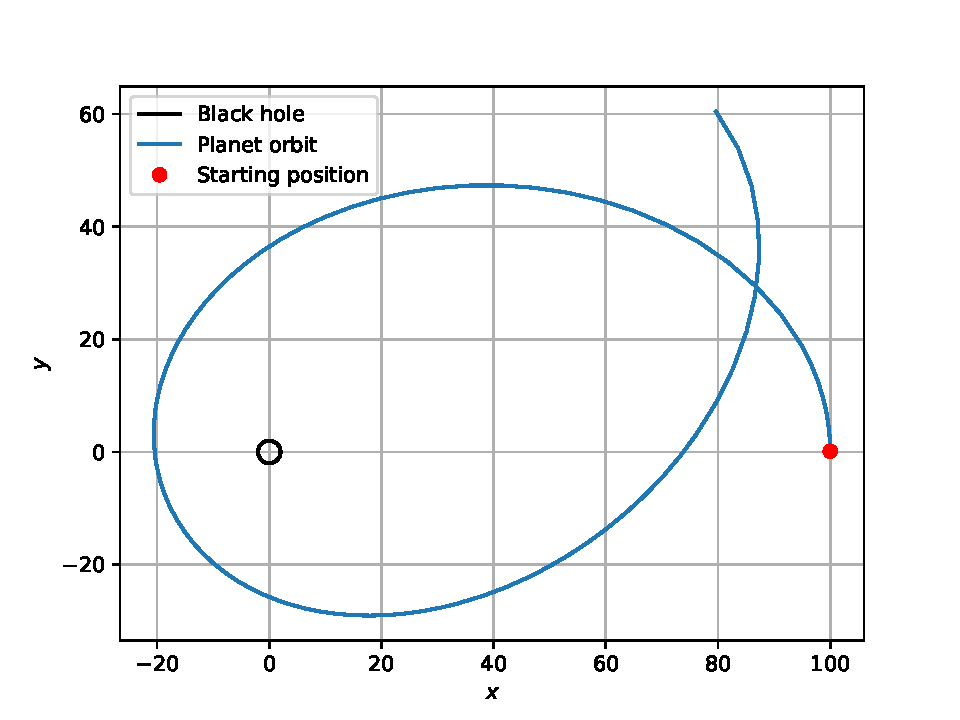
\includegraphics[scale=1]{./figs/planetOrbit.pdf}
			\caption{Orbit of a planet starting at $r = 100Rs$ and with velocity $v_\phi = 0.00075$. The perihelion precession of the elliptical orbit is observed as expected.}
			\label{orbit}
		\end{figure}
		
		The stepsize of the integration is determined by the ration of the error of components to the square norm of $y$. An independent way of checking accuracy is to check if the lorentzian length of the tangent vector is constant. In nonrelativistic mechanics problems energy conservation provides the possibility of independent verification of precision. Figure \ref{error}. shows the velocity squared ($\tensor{v}{^\mu}\tensor{v}{_\mu}$) as a function of integration steps.
		\begin{figure}[H]
			\centering
			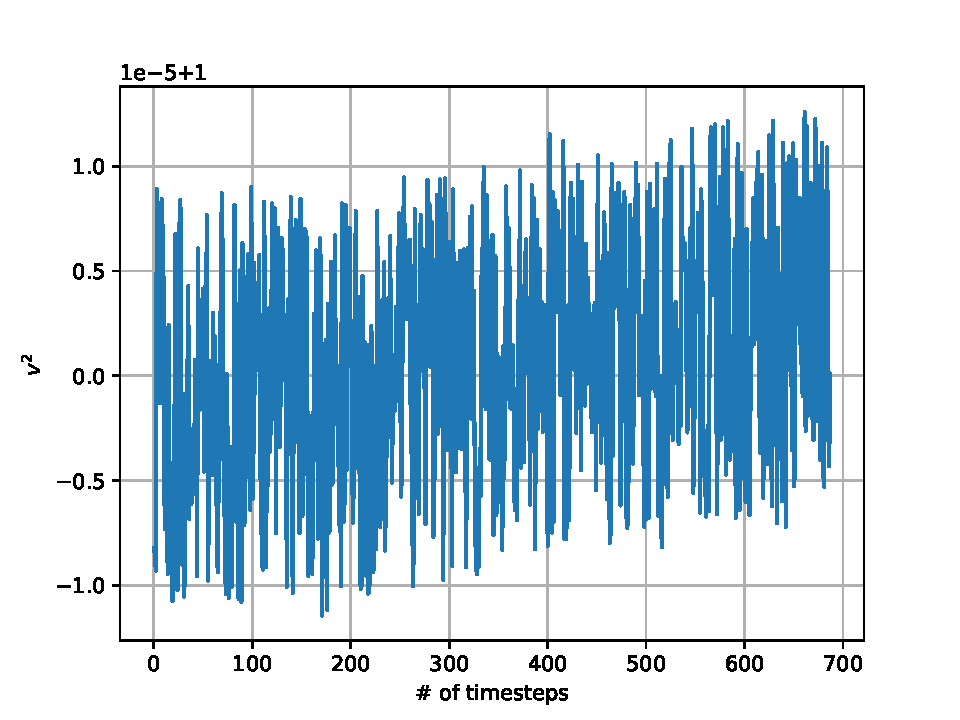
\includegraphics[scale=1]{./figs/planetError.pdf}
			\caption{The 4-velocity squared of the planet as a function of integration steps. With these tolerance settings of the integrator the relative error stays on the order of $10^{-5}$ even after over a dozen orbits.}
			\label{error}
		\end{figure}
		The velocity squared is on the order of $1\pm10^{-5}$ at the end of the simulation, after multiple orbits. Light rays rarely make more than a couple orbits around black holes, only for very specific angles, hence we expect this level of accuracy or better for the light rays used for the images.
		
		Finally it is interesting to look at the stepsize of the integration. This is shown on figure \ref{stepsize}.
		\begin{figure}[H]
			\centering
			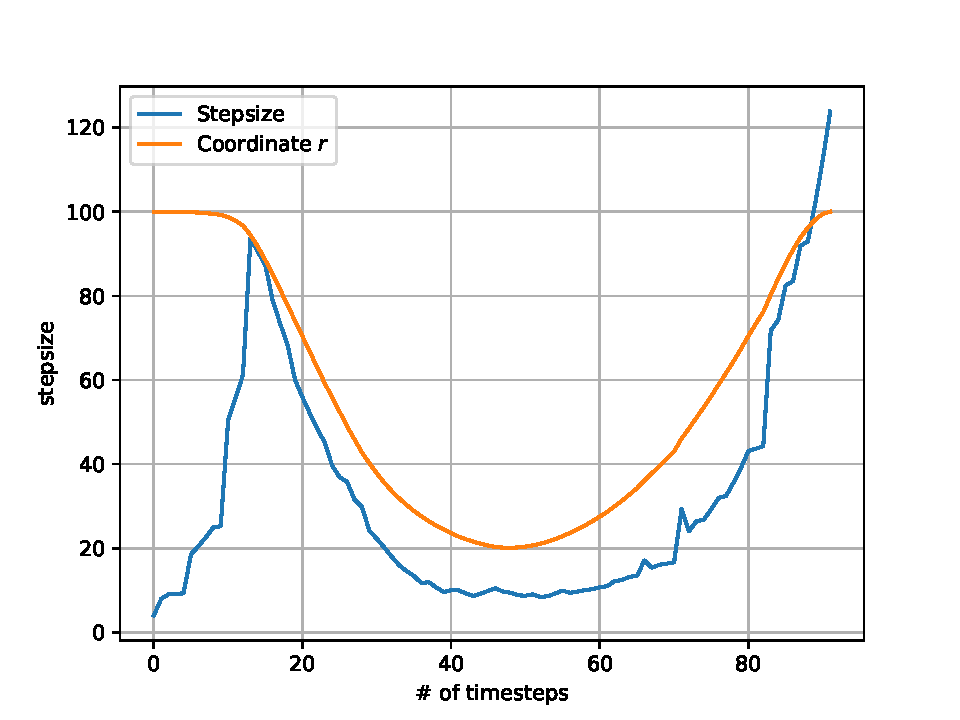
\includegraphics[scale=1]{./figs/planetStepsize.pdf}
			\caption{The stepsize of the integration as a function of the number of steps.}
			\label{stepsize}
		\end{figure}
		It can be seen that the stepsize grows exponentially until it reaches the optimal stepsize for the settings of the integrator. From then on it oscillates periodically roughly as a function of the $r$ coordinate. The curvature of the spacetime in the Schwarzschild solution is purely a function of the $r$ coordinate, so apart from the artifacts of the coordinate system (for example near the singularities in $\theta$). Therefore it is expected that for a given local precision the stepsize is a function of the $r$ coordinate. It is worth noting that this simulation consists of 688 time steps, and it was not necessary even one time to redo a timestep due to to the predicted timestep not being accurate enough.
	\subsubsection{Angle correction}
		\begin{figure}[H]
			\centering
			\begin{tabular}{c}
				\subcaptionbox{Checkerboard based on the corrected angles}{\centering 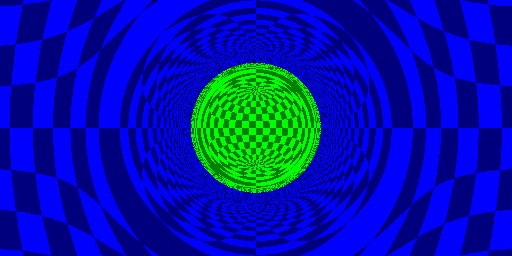
\includegraphics[scale=1.75]{./figs/angleCorrected.pdf}}\\
				\subcaptionbox{Checkerboard based on the angles without correction}{\centering 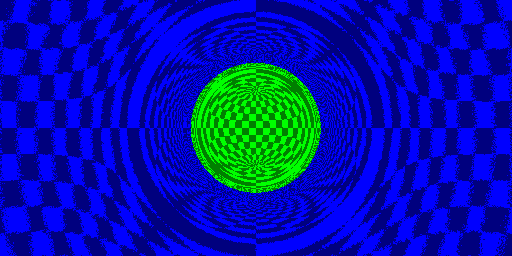
\includegraphics[scale=1.75]{./figs/angleNotCorrected.pdf}}
			\end{tabular}
			\caption{An image with and without the angle correction step after the collision is determined.}
			\label{anglecorrection}
		\end{figure}
		As expected the angle corrected version is a much clearer and more accurate image. The reason for the fuzzy edges in the image without angle correction is that the endpoints of the integration of each ray has a little randomness. The reason is that stepsize is finite, and the so the distance traveled after the true intersection with the outer sphere will vary. This causes the estimated angles to also vary a bit, leading to fuzzy edges.
	\subsubsection{Redshift}
		\begin{figure}[H]
			\begin{tabular}{cc}
				\subcaptionbox{Forward facing camera.}{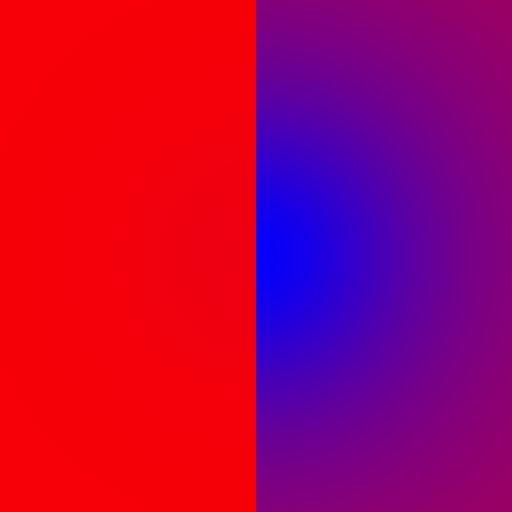
\includegraphics[scale=0.9]{./figs/frontRedshift.pdf}}&
				\subcaptionbox{Backwards facing camera.}{
\includegraphics[scale=0.9]{./figs/backRedshift.pdf}}\\
				\subcaptionbox{Outwards facing camera.}{
\includegraphics[scale=0.9]{./figs/outRedshift.pdf}}&
				\subcaptionbox{Sideways facing camera.}{
\includegraphics[scale=0.9]{./figs/sideRedshift.pdf}}
			\end{tabular}
			\caption{Images from a camera moving at relativistic speeds in the photon sphere and facing in different directions representing the amount of redshift observed.}
			\label{redshift}
		\end{figure}
		The cameras in figure \ref{redshift} are all moving at the same speed with no radial velocity component, located at the photon sphere. The red and green colors represent the amount of redshift in the direction of each pixel. The event horizon is expected to be a straight line here, because at the photon spheres light can orbit the black hole. Whether or not the light ray falls into the black hole or not depends entirely on the elevation with respect to the event horizon, resulting in the aforementioned straight line. In the pictures except the third one the solid red regions correspond to the event horizon. Light coming from there is infinitely redshifted. In the simulation this redshift is a finite value mainly determined by how close the light rays get to the event horizon before the simulation is terminated.
	\section{Conclusion}
		During the project we wrote a program capable of general relativistic ray tracing. In our opinion the main value of this program is pedagogycal. The program can be used to accurately illustrate what relativistic (both special and general) look like, and forces anybody who delves into the logic behind it to think about the real meaning of general relativity: the final step is not obtaining a solution to Einstein's equations, but to calculate what that solution implies about observations. This final step is often neglected especially when introducing the technical details. This program would be useful to illustrate pure special relativistic effects, although specialized solutions would be much faster.
		
		The results of the program agreed with expectations. Using an Intel Core i3 processor 1024x1024 light rays can be traced in around 20 seconds in Schwarzschield spacetime. This could be further improved by specializing the differential equation solver, at the moment it is a general algorithm implementing any explicit Runge-Kutta method.
	\bibliographystyle{abeld}
    \bibliography{ref}
\end{document}








